\documentclass[12pt, a4paper, openany]{report}

\def\VersionRapport{1.0}

\usepackage[utf8]{inputenc} % un package
\usepackage[T1]{fontenc}      % un second package
\usepackage[francais]{babel}  % un troisième package
\usepackage{layout}
\usepackage[top=2.7cm, bottom=2.5cm, left=3.5cm, right=3cm]{geometry}
\usepackage{setspace}

\frenchbsetup{StandardLists=true} % à inclure si on utilise \usepackage[french]{babel}
%\usepackage{enumitem}
\usepackage[shortlabels]{enumitem}
\usepackage{amssymb}

\usepackage{color}
\usepackage{listings}
\definecolor{dkgreen}{rgb}{0,0.6,0}
\definecolor{gray}{rgb}{0.5,0.5,0.5}
\definecolor{mauve}{rgb}{0.58,0,0.82}

\lstset{frame=tb,
  language=Java,
  aboveskip=3mm,
  belowskip=3mm,
  showstringspaces=false,
  columns=flexible,
  basicstyle={\small\ttfamily},
  numbers=none,
  numberstyle=\tiny\color{gray},
  keywordstyle=\color{blue},
  commentstyle=\color{dkgreen},
  stringstyle=\color{mauve},
  breaklines=true,
  breakatwhitespace=true,
  tabsize=3
}

\usepackage{multirow} % pour les tableaux
\usepackage[table]{xcolor} % pour les tableaux

\usepackage{verbatim}
\usepackage{moreverb}
\usepackage{url}
\usepackage{pst-all}
\usepackage{eso-pic,graphicx}
\usepackage{caption} 
\usepackage[colorlinks=true,urlcolor=blue,linkcolor=red]{hyperref}
\usepackage{array}
\usepackage[toc,page]{appendix}
\usepackage[off]{auto-pst-pdf}
\usepackage{hyperref} % pour le sommaire table des matières
\AddThinSpaceBeforeFootnotes % à insérer si on utilise \usepackage[french]{babel}
\FrenchFootnotes % à insérer si on utilise \usepackage[french]{babel}
\usepackage{fancyhdr}
\pagestyle{headings}
\usepackage{pifont}  %pour les puces
\usepackage{amsmath} %pour les puces

\usepackage{verbatim} % pour le code en annexe 

%%%%%%%colones 
\newcolumntype{R}[1]{>{\raggedleft\arraybackslash }b{#1}}
\newcolumntype{L}[1]{>{\raggedright\arraybackslash }b{#1}}
\newcolumntype{C}[1]{>{\centering\arraybackslash }b{#1}}
%%%%%%% 

\renewcommand{\appendixpagename}{Annexes}
\renewcommand{\appendixtocname}{Annexes}

\title{Theme: Compte Rendu Système Linéaire à Temps Continu 1}
\author{REBOUT \bsc{Mehenna}}
\author{BOUYOUCEF \bsc{Farid}}
\date{2018-2019}



%new
\newcommand{\HRule}{\rule{\linewidth}{0.5mm}}


\begin{document}

%\selectlanguage{francais}
\pagenumbering{arabic} 

\makeatletter
  \begin{titlepage}
  

  \begin{sffamily}
   \begin{center}

    % Upper part of the page. The '~' is needed because \\
    % only works if a paragraph has started.
    
\includegraphics[scale=0.5]{Logo_UT3.jpg}~\\[1.5cm]

    \textsc{\LARGE Master 1 EEA ISTR/RODECO  }\\[2cm]

    \textsc{\Large Compte Rendu  Système Linéaire à Temps Continu 1}\\[1.5cm]

    % Title
    \HRule \\[0.4cm] % saut de ligne
    { \huge \bfseries TP 1 Pendule\\[0.4cm] }

    \HRule \\[1cm]   % sous de ligne 
    
\includegraphics[scale=0.1]{logomaster.jpg}
    \\[1cm]

    % Author and supervisor
    \begin{minipage}{0.4\textwidth}
      \begin{flushleft} \large
         \textsc{\emph {Réalisés par:} \\REBOUT Mehenna}\\
         \textsc{BOUYOUCEF Farid}   
          \newline
          Promotion 2018-2019 \\
      \end{flushleft}
    \end{minipage}
    \begin{minipage}{0.4\textwidth}
      \begin{flushright} \large
        \emph{Tuteur :}  \textsc{M DUROLA}\\
        \emph{Responsable de la Formation:} \textsc{M GOUAISBAUT}
      \end{flushright}
    \end{minipage}

    \vfill

    % Bottom of the page
    {\large Octobre 2018}

  \end{center}
  \end{sffamily}      
          
  \end{titlepage}
  
\makeatother




   
%*********************** somaire **************
\renewcommand{\contentsname}{Sommaire}
\tableofcontents
%*********************** listes des figures **************
\listoffigures
%*********************** listes des tableaux **************
\listoftables



%*********************** INTRODUCTION **************
\chapter*{Introduction}
\addcontentsline{toc}{chapter}{Introduction}

\paragraph{Présentation du pendule inversé :} La Figure 1 donne une représentation schématique du pendule. Le bras est relié au moteur, qui entraîne la rotation du bras et donc du pendule. Il a une longueur L{r} et un moment d'inertie J{r} . Nous noterons son angle $\theta$ . Le pendule, quant à lui, est axé au bout du bras. Il a une longueur L{p}. Son moment d'inertie au centre de masse est noté J{p}. On note l'angle que fait l'axe du pendule avec l'axe verticale a (en radian).

\begin{center}
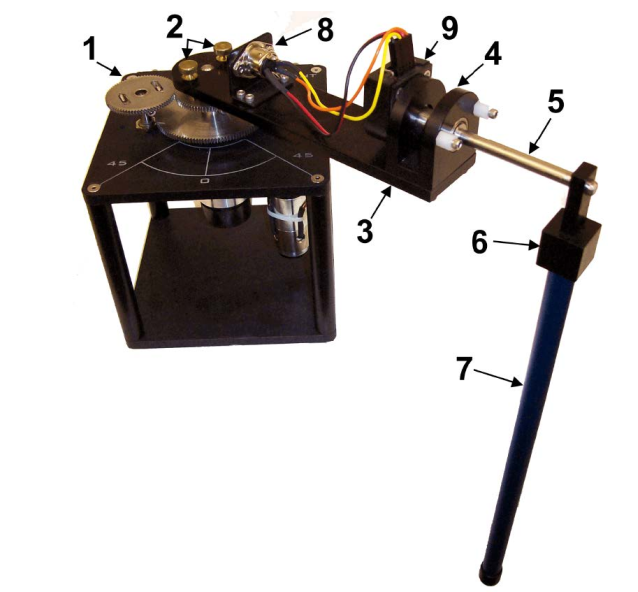
\includegraphics[scale=0.5]{pondule.png}
\captionof{figure}{\textit{Composant du pendule}}
\label{fig1} 
\end{center}

\paragraph{Précision du lieu :} Ce TP a eu lieux a l’université Paul SABATIER dans la salle TP I3.   

\paragraph{La date :} Ce sujet nous a été attribué par M DUROLA le mois d'octobre  et on va le rendre le 19/11/2018 à M DUROLA.

\paragraph{But de la manipulation :}  Dans cette manipulation on se propose de réaliser un asservissement permettant la régulation du pendule inversé représentée par la Figure 1.1 en position haute comme le montre la Figure 1.2. On utilisera pour cela les techniques d'espace d'état à temps continu. Cette manipulation est constituée de quatre grandes étapes : modélisation, analyse, régulation et implémentation. Les objectifs du TP sont les suivants :
\begin{itemize}
\item Savoir établir un modèle linéarisé autour d'un point d'équilibre.
\item Savoir établir les propriétés structurelle d'un système linéaire.
\item Savoir utiliser Matlab et sa toolbox simulink.
\item Savoir synthétiser une commande par retour d'état.
\item Savoir faire la simulation de modèles linéaires et non linéaires.
\item Savoir utiliser les différentes commandes MATLAB pour étudier un système.

\end{itemize}

    
    %******************* MODÉLISATION **********
 \chapter{Modélisation}
 
 La Figure 1.1 donne une représentation schématique du pendule. Le bras est relié au moteur, qui entraîne la rotation du bras et donc du pendule. Il a une longueur $L_{r}$ et un moment d'inertie $J_{r}$. Nous noterons son angle $\theta$.\\
 Le pendule, quant à lui, est lixé au bout du bras. Il a une longueur $L_{p}$ . Son moment d'inertie au
centre de masse est noté $J_{p}$. On note l'angle que fait l'axe du pendule avec l'axe verticale $\alpha$ (en radian).\\
 Tous les calculs de la modélisation se feront en prenant pour origine, la position haute du pendule. pour les descriptions et les valeurs numériques des constantes se reporter à la Table (num du table....) \\
 Les équations du mouvement, déterminées à l'aide de la mécanique Lagrangienne, sont données par les
deux équations différentielles suivantes : \\[1cm]\\

 %\big(a+b \big) \\ 
 %\bigg(a+b+c \bigg) \\
 %\Big(a+b+c+d \Big)\\
 %\Bigg(a+bjhbnjkhnkjn \Bigg)\\
     

  $\bigg(m_{p}L_{r}^{2} + \frac{1}{4}m_{p}L_{p}^{2} - \frac{1}{4}m_{p}L_{p}^{2}cos(\alpha^{2}) + J_{r} \bigg)$ $\ddot{\theta}$

   


\section{Étude succinte du modèle non linéaire  }

                                                 


%%%%%%%%%%%%%%%%%%%%%%%%% Tableau%%%%%%%%%%%%%%%%%%%ù


\begin{center}
%\begin{tabular}{|R{2cm}|C{8cm}|L{2.5cm}|}
\begin{tabular}{|l|c|r|}
\hline \rowcolor{lightgray} Symbole & Description &  Valeur  \\
\hline  $B_{p}$  &  Coefficient de frottement visqueux du pendule  & $0.0024 kg/m^{2}$   \\
\hline  $B_{r}$ & Coefficient de frottement visqueux du bras & $0.0024 kg/m^{2}$ \\
\hline  $\eta_{g}$  &  Rendement du réducteur  & $0.9$  \\

\hline 
\end{tabular}
\captionof{table}{Liste des données spécifique au système}
\end{center}


%%%%%%%%%%%%%%%%%%%%%%%%%%%%%%%%%%%%%%%




 %\begin{enumerate}[(a)]
  % \item Le système sera stable en boucle fermée
   %\item Une erreur de position nulle
   %\item Une erreur de vitesse limitée à 1 i.e. lorsque l'entrée de consigne est une rampe de pente 1
   %\item Une convergence vers la consigne en moins de 3 seconde, sans oscillations, ni dépassement.
   %ù\item Un rejet de la perturbation de fuite.
   %ù\item Un rejet du bruit de mesure au-delà de 100 Hz d’au moins de 60 dB par.
 %\end{enumerate}
	
%*********************** Problématique **************
\chapter{Analyse temporelle et structurelle du modèle linéarisé }
 %\chaptermark{Cmd proportionnelle intégrales} (pour avoir ce titre en petit 
\begin{center}
\begin{tabular}{|R{2cm}|C{8cm}|L{2.5cm}|} 
\hline \rowcolor{lightgray} Symbole & Description &  Valeur  \\
\hline  \begin{center} $B_{p}$\end{center}  &  \begin{center}Coefficient de frottement visqueux du pendule\end{center}  & \begin{center}$0.0024 kg/m^{2}$ \end{center}  \\
\hline  \begin{center} $B_{r}$\end{center} & \begin{center}Coefficient de frottement visqueux du bras\end{center} & \begin{center}$0.0024 kg/m^{2}$ \end{center}\\
\hline  \begin{center} $\eta_{g}$\end{center}  &  \begin{center}Rendement du réducteur\end{center}  & \begin{center}$0.9$ \end{center}  \\
\hline  \begin{center} $\eta_{m}$\end{center}  &  \begin{center}Rendement du moteur\end{center}  & \begin{center}$0.69$ \end{center}  \\
\hline  \begin{center} $K_{g}$\end{center}  &  \begin{center}Rapport de vitesse\end{center}  & \begin{center}$70$ \end{center}  \\
\hline  \begin{center} $K_{m}$\end{center}  &  \begin{center}Gain f.e.m\end{center}  & \begin{center}$7.68*10^{-3} V/(rad/s)$ \end{center} \\
\hline  \begin{center} $K_{t}$\end{center}  &  \begin{center}Gain couple moteur/courant\end{center}  & \begin{center}$7.68*10^{-3} N.(m/A)$ \end{center}\\
\hline  \begin{center} $J_{p}$\end{center}  &  \begin{center}Moment d'inertie du pendule au centre dde masse \end{center}  & \begin{center}$0.0012 kg/m^{2}$ \end{center}\\
\hline  \begin{center} $J_{r}$\end{center}  &  \begin{center}Moment d'inertie du bras au centre dde masse \end{center}  & \begin{center}$9.98*10^{-4} kg/m^{2}$ \end{center}\\
\hline  \begin{center} $L_{m}$\end{center}  &  \begin{center} Inductance du moteur \end{center}  & \begin{center}$0.18 mH$ \end{center}\\
\hline  \begin{center} $L_{p}$\end{center}  &  \begin{center} longueur du pendule \end{center}  & \begin{center}$0.337 m$ \end{center}\\
\hline  \begin{center} $L_{r}$\end{center}  &  \begin{center} Inductance du bras, du pivot à l'extrémité \end{center}  & \begin{center}$0.216 m$ \end{center}\\
\hline  \begin{center} $m_{p}$\end{center}  &  \begin{center} Masse du pendule \end{center}  & \begin{center}$0.127 kg$ \end{center}\\
\hline  \begin{center} $m_{r}$\end{center}  &  \begin{center} Masse du bras \end{center}  & \begin{center}$0.257 kg$ \end{center}\\
\hline  \begin{center} $R_{m}$\end{center}  &  \begin{center} Résistance du moteur \end{center}  & \begin{center}$2.60 \Omega$ \end{center}\\
\hline  \begin{center} $V_{m}$\end{center}  &  \begin{center} Tension envoyé au moteur \end{center}  & \begin{center} A régler \end{center}\\
\hline 
\end{tabular}
\captionof{table}{Liste des données spécifique au système} 
 \end{center}
 
 %pour espace    \hspace{2mm}
 
 


% *********************** Conclusion *****************
\chapter*{Conclusion}
\addcontentsline{toc}{chapter}{Conclusion}

Ce TP nous a permet d'utiliser les différentes commandes de robustesse et a appris de définir un correcteur par étapes, cela en vérifiant chaque contrainte pour déterminer un meilleur correcteur.\\




 %\chapter*{Annexe}
% \addcontentsline{toc}{chapter}{Introduction}

% CODE MATLAB


%\begin{verbatim}



 

% \end{verbatim}






%Bibliographie 
%\bibliographystyle{alpha}
%\bibliography{biblio}



\end{document}





